\section{Two-Moment Model}

\subsection{Transport Equations}
Considering some massless fermion pass through a static material and only emission, absorption and elastic scattering exist, the transport equation of the fermion after scaling to dimensionless units can be written as
\begin{equation}
  \pd{f}{t}+\vect{\ell}\cdot\nabla f
  =\f{1}{\tau}\,\cC(f).
  \label{eq:boltzmann}
\end{equation}
whic is known as Boltzmann equation.
The distribution function $f = f(\omega,\varepsilon,\vect{x},t)$ gives the number of particles propagating in the direction $\omega\in\bbS^{2}$, with energy $\varepsilon\in\bbR^{+}$, at position $\vect{x}\in\bbR^{3}$ and time $t\in\bbR^{+}$.  
$\vect{\ell} = \vect{\ell}(\omega)\in\bbR^{3}$ is the unit vector which parallel to the fermion three-momentum direction: $\vect{p}=\varepsilon\,\vect{\ell}$.
On the right-hand side, $\tau$ is interaction strength parameter: $\tau\ll1$ for opaque (strong interaction with the background) region while $\tau\gg1$ for transparent (weak interaction with the background, or free streaming) region.
$\cC(f)$ is the collision term, which models emission, absorption, and isotropic and elastic scattering: 
\begin{equation}
  \cC(f)=\xi\,\big(\,f_{0}-f\,\big)
  +(1-\xi)\,\big(\,\f{1}{4\pi}\int_{\bbS^{2}}f\,d\omega-f\,\big),
  \label{eq:collisionTerm}
\end{equation}
where $\xi$ is the emission and absorption contribution parameter: $\xi = 1$ for pure emission and absorption, or no scattering; $\xi = 0$ for pure scattering. 
$f_{0}$ is the fermion equilibrium distribution function which has the following form:
\begin{equation}
  f_{0}(\vect{z})=\f{1}{e^{(\varepsilon-\mu(\vect{x}))/T(\vect{x})}+1},  
  \label{eq:fermiDirac}
\end{equation}
where $T$ is the temperature in energy unit, and $\mu$ is the fermion chemical potential.
Both of them depend on the properties of the background.

\subsection{Two-Moment Model}
An approximate solution of Boltzmann equation Eq.~\eqref{eq:boltzmann} can be found by using two-moment model.
In two-moment model, the angular moments of the distribution function are defined as
\begin{equation}
  \big\{\,\cJ,\vect{\cH},\vect{\cK}\,\big\}(\vect{z},t)
  =\f{1}{4\pi}\int_{\bbS^{2}}f(\omega,\vect{z},t)\,\{\,1,\vect{\ell},\vect{\ell}\otimes\vect{\ell}\,\}\,d\omega.  
  \label{eq:angularMoments}
\end{equation}
with $\vect{z}:=\{\varepsilon,\vect{x}\}$.
The zeroth moment $\cJ$ is referred as the particle density, while the first moment $\bcH$ the particle flux and the second moment $\bcK$ the stress tensor.
Besides, define $\vect{\cM}=(\cJ,\vect{\cH})^{T}$ and $\vect{\cF}=(\vect{\cH},\vect{\cK})^{T}$, then take the zeroth and first moment of Eq.~\eqref{eq:boltzmann}, we have
\begin{equation}
  \pd{\vect{\cM}}{t}+\nabla\cdot\vect{\cF}=\f{1}{\tau}\,\vect{\cC}(\vect{\cM}),
  \label{eq:momentEquations}
\end{equation}
with
\begin{equation}
  \vect{\cC}(\vect{\cM})=\vect{\eta}-\vect{\cD}\,\vect{\cM},
  \label{eq:collisionTermMoments}
\end{equation}
where $\vect{\eta}=(\xi\,f_{0},\vect{0})^{T}$ and $\vect{\cD}=\mbox{diag}(\xi,\vect{I})$.
$\vect{I}$ is the identity matrix.  

\subsection{Algebraic Closures }
To close the system given by Eq.~\eqref{eq:momentEquations}, a strategy named algebraic closure is used.
Algebraic closures give approximate $\bcK$ based on the lower moments:
\begin{equation}
\bcK = \vect{k} \cJ,
\end{equation}
where $\vect{k}$ is the Eddington tensor.
Levermore\cite{levermore_1984} assumed that the radiation field is symmetric about a preferred direction $\widehat{\vect{h}}=\vect{\cH}/|\vect{\cH}|$ and gave 
\begin{equation}
  \vect{k}=\f{1}{2}\big[\,\big(1-\chi\big)\,\vect{I}+\big(3\,\chi-1\big)\,\widehat{\vect{h}}\otimes\widehat{\vect{h}}\,\big],
  \label{eq:eddingtonTensor}
\end{equation}
where $\chi=\chi(\cJ,|\vect{\cH}|)$ is the Eddington factor. 

\subsection{Constraints on Moments}
One fundamental fact one should concern before solving the system is the property he/she should never violate.
For a fermionic system, the property is Pauli exclusion principle, or 
\begin{equation}
f \in (0,1).
\end{equation}
As a result, the angular moments as the integrations of $f$ are confined as following
\begin{align}
\cJ \in(0,1), \quad &(1-\cJ)\cJ-|\vect{\cH}|  > 0, \\
  \chi_{\mbox{\tiny min}}
  =\max\big(1-\f{2}{3\cJ},h^{2}\big)
  < & \chi<\min\big(1,\f{1}{3\cJ}-\f{\cJ}{1-\cJ}h^{2}\big)=\chi_{\mbox{\tiny max}},
  \label{eq:eddingtonFactorBounds}
\end{align}
where $h = |\bcH|/\cJ$ is the flux factor.
As Fig.~\eqref{fig:EddingtonFactorsWithDifferentClosure} shows, not all the algebraic closures satisfy the constraints on moments all the time: Kershaw [citation], Wilson [citation], Levermore [citation], Minerbo [citation], Janka 2 [citation] may work fine at low occupancy case, but not at high occupancy situation; Janka 1 [citation] is even worse and not work all the time. Only Cernohorsky \& Bludman[citation] among these plotted closures remains in the realizable region.
\begin{figure}[h]
  \centering
  \begin{tabular}{cc}
    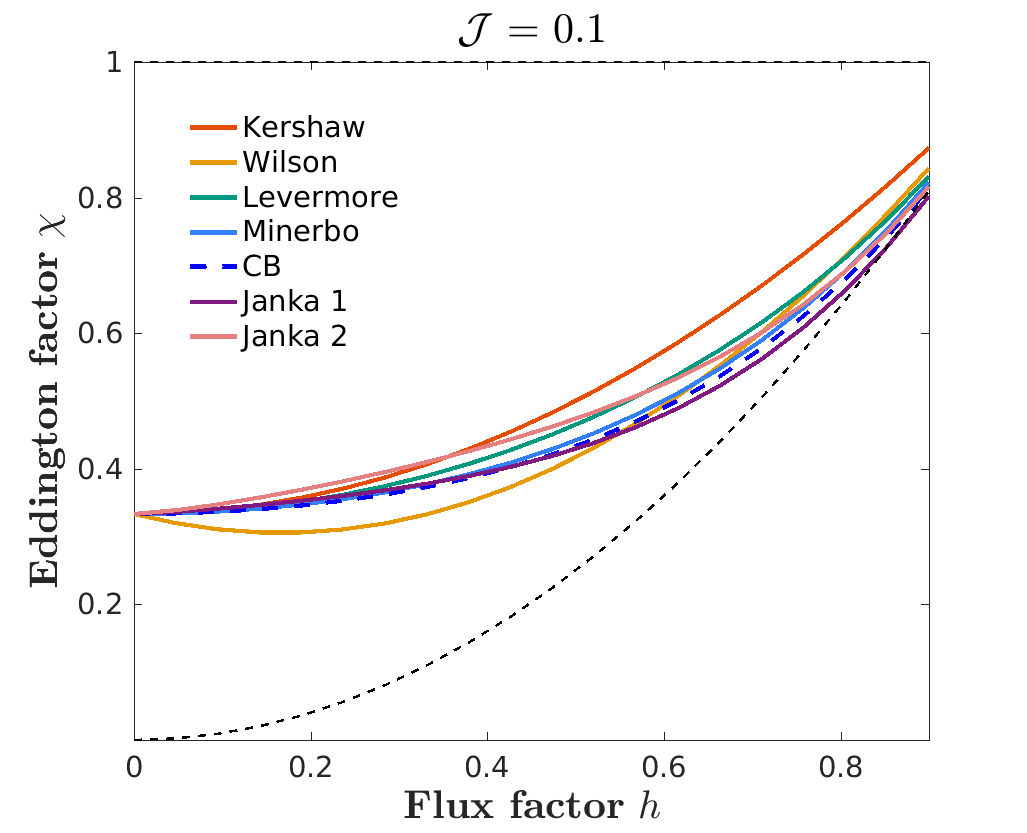
\includegraphics[width=0.5\textwidth]{figures/Closures0_10}
    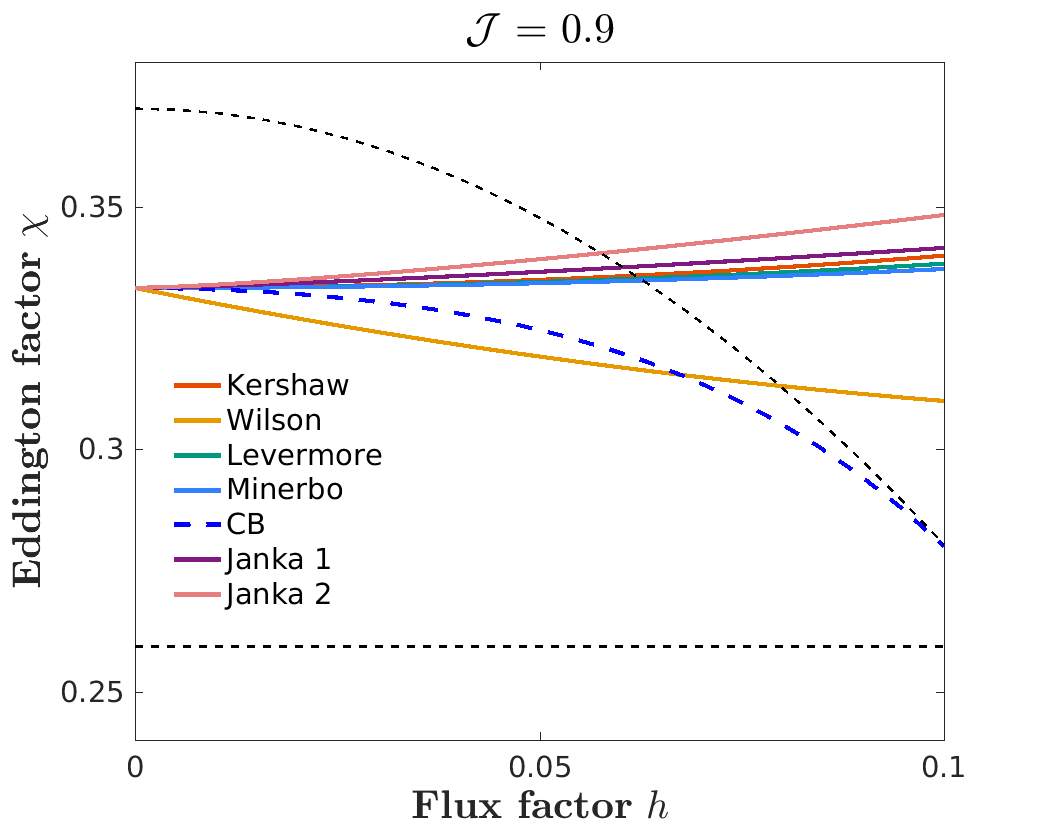
\includegraphics[width=0.5\textwidth]{figures/Closures0_90}
  \end{tabular}
   \caption{Plot of Eddington factors $\chi$ versus flux factor $h$ for different values of $\cJ$ for various algebraic closures: $\cJ=0.1$ (left panel, low occupied) and $\cJ=0.9$ (right panel, high occupied).  In each panel we plot the Eddington factors of Kershaw (red), Wilson (yellow), Levermore (green), Minerbo (light blue), Cernohorsky \& Bludman (blue) and Janka (purple and pink) closures.  We also plot $\chi_{\mbox{\tiny min}}$ and $\chi_{\mbox{\tiny max}}$ defined in Eq.~\eqref{eq:eddingtonFactorBounds} (lower and upper dash black lines, respectively).}
  \label{fig:EddingtonFactorsWithDifferentClosure}
\end{figure}

